% classes
\documentclass{article}

% packages
\usepackage{graphicx}
\usepackage{fancyhdr} % Required for custom headers
\usepackage{lastpage} % Required to determine the last page for the footer
\usepackage{extramarks} % Required for headers and footers
\usepackage{courier} % Required for the courier font

\usepackage{color}
\usepackage{enumitem}

\usepackage{hyperref}


% page layout


\topmargin=-0.45in
\evensidemargin=0in
\oddsidemargin=0in

\textwidth=6.5in
\textheight=9.0in

\headsep=0.25in

\linespread{1.1} % Line spacing
 
\pagestyle{fancy}

% headers and footers

\fancyhf{}

\lhead{INTR 100 Breaking Intuition}

\rhead{
\includegraphics[width=0.045\textwidth]{wmlogo.jpg}}



% document body

\begin{document}

\vspace*{.01mm}

\begin{center}

\Large{\textcolor{blue}{\textbf{Lab 5.}  Reimagining New York City}}

\vspace{4mm}

\textit{Due by noon on Friday, November 13th}\\

\end{center}

\begin{figure}[h!]
\begin{center}
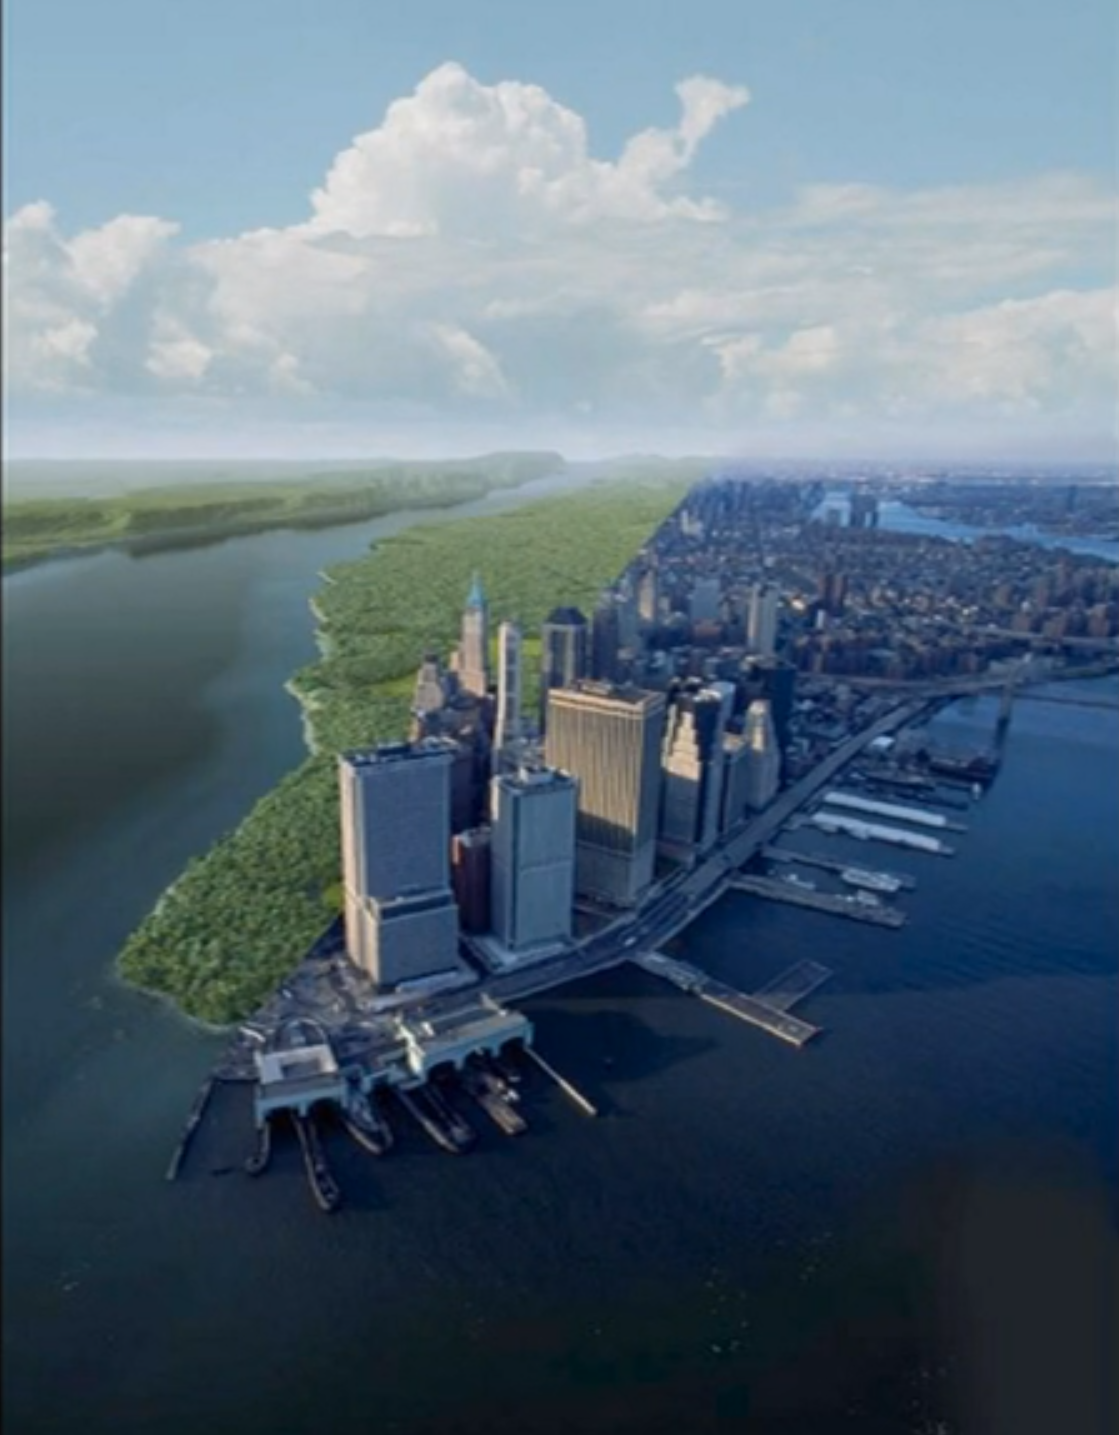
\includegraphics[width=0.75\textwidth]{nyc.png}

\end{center}
\end{figure}

\setlength{\parindent}{0cm}

\large{\textit{"And as the moon rose higher the inessential houses began to melt away until gradually I became aware of the old island here that flowered once for Dutch sailors' eyes - a fresh, green breast of the new world."}
\begin{flushright}
from Chapter 9 of F. Scott Fitzgerald's, The Great Gatsby
\end{flushright}
}


\newpage

% Enumerate the Laboratory Objectives

\large{\textbf{Laboratory in Brief:}}

\vspace{4mm}

\setlength{\leftskip}{1cm}

\setlength{\parindent}{0cm}

The purpose of this laboratory is to use the Visionmaker NYC, vision-making application to develop a future vision of New York City.  By focusing on the interconnected social services and infrastructure including stormwater management; climate change adaptation and mitigation; brownfield remediation; air, water, noise, and soil pollution; invasive species and disease; and habitat deterioration and destruction you will create a vision of New York City that addresses ecological  limitations and quality of life in the city. Your goal is to address environmental challenges through which New Yorkers may come to recognize and embrace the special qualities of place that has been woven into the nature?s tapestry, thus opening new avenues for design, development, art, science, economy and sustainability.

\vspace{4mm}

\setlength{\leftskip}{0cm}

\large{\textbf{Specific Objectives:}}

\begin{enumerate}[leftmargin=15mm]

\item To use the Vision Maker New York City to define a vision extent and chose a life style and climate for building a scenario to model.

\item To use the ecosystem tool palette to select ecosystems and modifiers to paint the ecosystems of the vision area.  

\item To creata a document that describes your Vision for New York City including spatial images that support your report.

\end{enumerate}

% Enumerate the Laboratory Objectives

\large{\textbf{Software and Resources you will need or will be helpful:}}

\begin{enumerate}[leftmargin=15mm]

\item Watch Eric Sanderson's June 2009 TED talk: New York - before the City \\  
\url{http://www.ted.com/talks/eric_sanderson_pictures_new_york_before_the_city}

\item Goto to the New York City Vision maker website, create an account and login.  The website may have compatibility issues with some web browsers; use Firefox or Google Chrome if you experience problems. \\ 
\url{https://visionmaker.us/nyc/}

\item Goto the project website, review the material available there, including the publications \\ 
\url{https://welikia.org}

\end{enumerate}


\newpage

\textbf{Grading}

\vspace{4mm}

\setlength{\leftskip}{1cm}

\setlength{\parindent}{0cm}

This lab will be graded in 2 parts.  \textbf{First}, you will create a vision for New York City using the VisionMaker NYC (35\%).  \textbf{Second}, you will use output from your Vision Maker NYC as documentation incorporated into your report (65\%). \\

Your lab report should include the following elements.

\begin{enumerate}[leftmargin=15mm]

\item Creation of a lifestyle, climate and precipitation scenarios for a chosen part of New York City.

\item Introduce your vision of New York City using the Ecosystem tools.  Higher grades will be reserved for work that has given more thoughtful consideration to built and natural ecosystems, transportation, ecosystem modifiers and other characteristics.

\item Using these elements produced by the Visionmaker New York City in support of your vision.

\end{enumerate}

\vspace{7mm}

\begin{figure}[h!]
\begin{center}
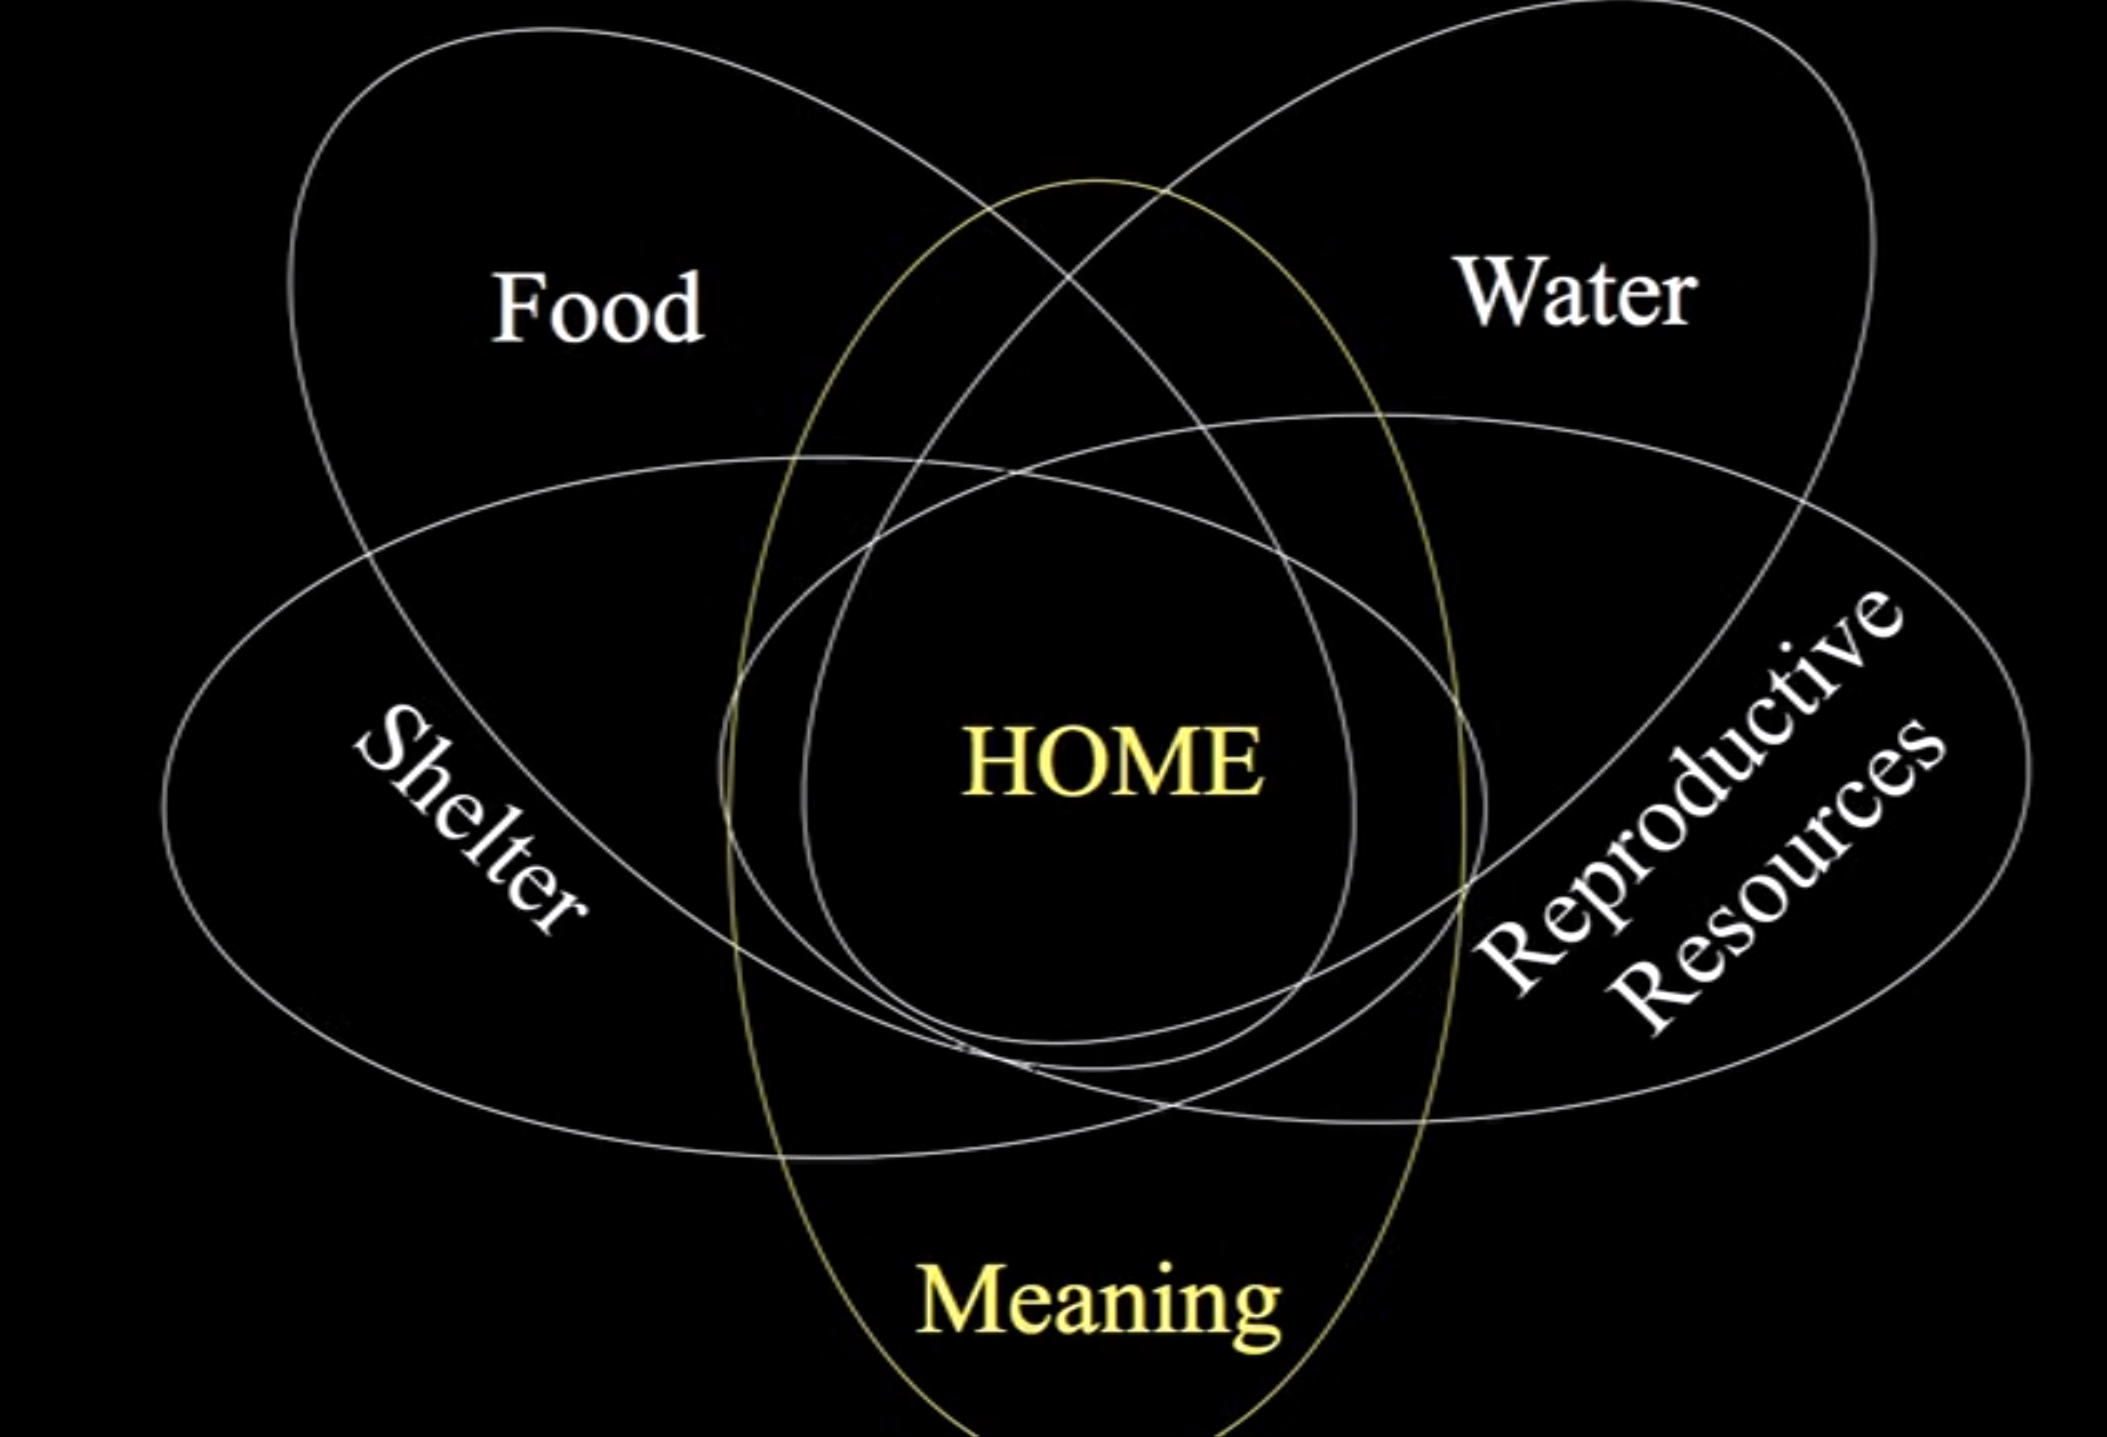
\includegraphics[width=0.7\textwidth]{home.png}

\end{center}
\end{figure}

\setlength{\leftskip}{0cm}

\normalsize{\textit{"Of all the strange things that Alice saw in her journey Through The Looking-Glass, this was the one that she always remembered most clearly. Years afterwards she could bring the whole scene back again, as if it had been only yesterday - the mild blue eyes and kindly smile of the Knight - the setting sun gleaming through his hair, and shining on his armour in a blaze of light that quite dazzled her - the horse quietly moving about, with the reins hanging loose on his neck, cropping the grass at her feet - and the black shadows of the forest behind - all this she took in like a picture, as, with one hand shading her eyes, she leant against a tree, watching the strange pair, and listening, in a half dream, to the melancholy music of the song."}
\begin{flushright}
\large{from Chapter 8 of Lewis Carroll's, Through the Looking-Glass}
\end{flushright}
}

%----------------------------------------------------------------------------------------

\end{document}